\documentclass[addpoints,12pt]{exam}
\usepackage{amsfonts}
\usepackage{amsmath}
\usepackage{fancyvrb}
\usepackage{multirow}
% commands are macros that we makeup to make our life easier
% \set, \Set, and \Nat can now be used with ease in the doc
% easier to type `\Nat` than `\mathbb{N}` when you need a fancy N shape - imo
\newcommand{\set}[1]{\left\{ #1 \right\}}
\newcommand{\Set}[1]{\big\{ #1 \big\}}
\newcommand{\Nat}{\mathbb{N}}
\newcommand{\TODO}[1]{{\color{orange}{TODO: #1}}}% SPWI: delete these
\newcommand{\Soln}[1]{{\color{red}{SOLUTION: #1}}}% SPWI: delete these
\newcommand{\SolnNo}{\Soln{No solutions provided for this sample, it is up to you to verify your understanding of the topic using the resources that are available to you. Ask your peers, use office hours, use \hyperlink{https://edstem.org/us/courses/72170/discussion}{EdStem}.}}

\newcommand{\Grade}[1]{{\color{brown}{GRADING CRITERIA: #1}}}% SPWI: change color and showingness.
\newcommand{\twocol}[2]{\begin{figure}[!htb]
    \centering
    \begin{minipage}{.5\textwidth}
    #1
    \end{minipage}%
    \begin{minipage}{0.5\textwidth}
     #2
    \end{minipage}
\end{figure}
}
\usepackage{color}
\usepackage{xcolor,pgf,tikz,pgflibraryarrows,pgffor,pgflibrarysnakes}
% https://www.overleaf.com/learn/latex/Hyperlinks#Linking_web_addresses
\usepackage{hyperref}
\hypersetup{
    colorlinks=true,
    linkcolor=blue,
    filecolor=magenta,      
    urlcolor=cyan,
    pdftitle={Overleaf Example},
    pdfpagemode=FullScreen,
    }


    
\usetikzlibrary{fit} % fitting shapes to coordinates
\usetikzlibrary{backgrounds} % drawing the background after the foreground

\usepgflibrary{shapes}
\usetikzlibrary{snakes}
\usetikzlibrary{automata,positioning} 
\usetikzlibrary{arrows.meta,automata,positioning,shadows} 

\tikzstyle{background}=[rectangle,fill=gray!10, inner sep=0.1cm, rounded corners=0mm]

\usepackage{tikz}
\tikzstyle{nloc}=[draw, text badly centered, rectangle, rounded corners, minimum size=2em,inner sep=0.5em]
\tikzstyle{loc}=[draw,rectangle,minimum size=1.4em,inner sep=0em]
\tikzstyle{trans}=[-latex, rounded corners]
\tikzstyle{trans2}=[-latex, dashed, rounded corners]
\definecolor{gold}{rgb}{0.83, 0.69, 0.22}
\newcommand{\Aa}{\mathcal{A}}

\addpoints
\boxedpoints

% \title{Programming and Data Structures (Midterm Exam 3)}
% \date{Midterm Exam 3}
\author{}
\begin{document}
% \maketitle

\pagestyle{headandfoot}
\runningheadrule
\firstpageheader{CSCI 1300: Spring 2025}{Finals Study Guide}{\today}
\runningheader{Finals Study Guide}
              {Name:}% TODO: your name in the block to be on the top of each page
              {}
              \firstpagefooter{}{}{\thepage}
              \runningfooter{}{}{\thepage}

\section{Background}
\textbf{The questions in this study guide are designed to be difficult and help you identify knowledge gaps that warrant further study.} By request, this study guide is compiled to help you prepare for final exams. Instruction during the final week of lecture may or may not cover sections of this packet. Please use this as you see fit. We hope this helps you prepare for your CSCI 1300 final exam and future studies. This packet does its best to cover all topics of the course, but is not exhaustive. Supplement with additional material as you see fit. 
\\
\\
We strongly recommend reviewing the following sections of your textbook "Brief C++ Late Objects" - Cay Horstmann, including the embedded "Self Check"s:

\begin{itemize}
    \item Chapter 1 subsections: 2 - 4
    \item Chapter 2 subsections: 1 - 3, 5
    \item Chapter 3 subsections: 1 - 7
    \item Chapter 4 subsections: 1 - 3, 5, 6, 8 - 10
    \item Chapter 5 subsections: 1 - 10
    \item Chapter 6 subsections: 1 - 7
    \item Chapter 7 subsections: 3, 7
    \item Chapter 8 subsections: 1 - 4
    \item Chapter 9 subsections: 1 - 6, 9, 11
\end{itemize}    
\\
Some solutions will be provided in a solution document.
\\
\Soln{Solutions \hyperlink{https://github.com/SpenceIsCool/cu-csci1300-sp25-wilson-code-samples/blob/main/Exams/final.cpp}{code available here}. Additional solutions in red in-situ.}
\\
\\
If you cannot think of a problem worth solving in the self-study section: ask a peer, ask a member of the course staff (in office hours or on EdStem), ask an AI that you trust. 
\\
\\
In general, you should think about the following tasks for any given self-study.
\begin{enumerate}
    \item Write out what you know about the topic. Identify what is tricky about this topic.
    \item Define a problem to solve: draw a cartoon of the problem, define some expected input and result, confirm that the defined problem will address whatever is tricky about the topic.
    \item After you have completed the work on paper, validate your work using your preferred coding environment. Prioritize paper studies first.
    \item Decide if you need to study this further and construct additional study materials.
\end{enumerate}
\newpage

\begin{questions}
\section{Compilation}
\question Compilation
    \begin{parts}
        \part What is the shortest command used to compile a file named \texttt{driver.cpp}?
            \\
            \Soln{\texttt{g++ driver.cpp}}
        \part What if \texttt{driver.cpp} has the line \texttt{\#include "className.h"}, following best practices for naming conventions, how do you correctly compile the driver file?
            \\
            \Soln{\texttt{g++ className.cpp driver.cpp} \\ observe that the compilation uses className.cpp, NOT className.h}
        \part What flags should you also consider using? What is the purpose of each compilation flag?
            \\
            \Soln{
                \begin{itemize}
                    \item \texttt{-std=c++17}: set the c++ standard to use [here 2017] (note that there are new standards every 3 years)
                    \item \texttt{-o whatever.o}: specifiy the name of the executable [here \texttt{whatever.o}], rather than \texttt{a.out} for Linux/Mac or \texttt{a.exe} for Windows
                    \item \texttt{-Wall -Werror -Wpedantic -Wsign-compare}: each of these are well detailed in this semesters \hyperlink{https://cu-csci-1300-intro-programming.github.io/spring-2025-web/jekyll/update/2025/04/01/Week-16-Final-Exam-Prep.html}{workbook}
                \end{itemize}
            }
        \part Given that you have compiled the code, how do you execute the code from the command line?
            \\
            \Soln{
                \begin{itemize}
                    \item LINUX/MAC: \texttt{./a.out}
                    \item Windows: \texttt{.\\a.exe}
                    \item custom: using the \texttt{-o} flag, you may speficy a different file
                \end{itemize}
            }
    \end{parts}
    \newpage
    
\question{Essentials::} For each of the following topics, in your own words: (1) define the principles of the topic (2) give one example of the topic (3) identify and explain any important nuances about the topic (4) decide for yourself if you need to study this particular topic further and seek resources for it (textbook, workbook, lecture documents, lecture videos, peers, EdStem, course staff, youtube, the open internet, and more). Use additional paper as needed.
    \begin{parts}
        \part essential types and their operations: bool, short, int, float, double, char, string
        \part conditions (if/else-if/else) and switches
        \part functions (pass-by-value vs pass-by-reference)
        \part loops
        \part arrays
        \part streams (input vs output) (\texttt{getline} vs \texttt{>>})
        \part structs/instances
        \part classes/objects
        \part vectors
        \part sorting
        \part recursion
    \end{parts}
    \\
    \SolnNo
    \newpage
    
\question{Writing Functions: Warm Up::} The questions on this page ask about the image provided (a function in graph form):    \\    
\begin{parts}
\twocol{
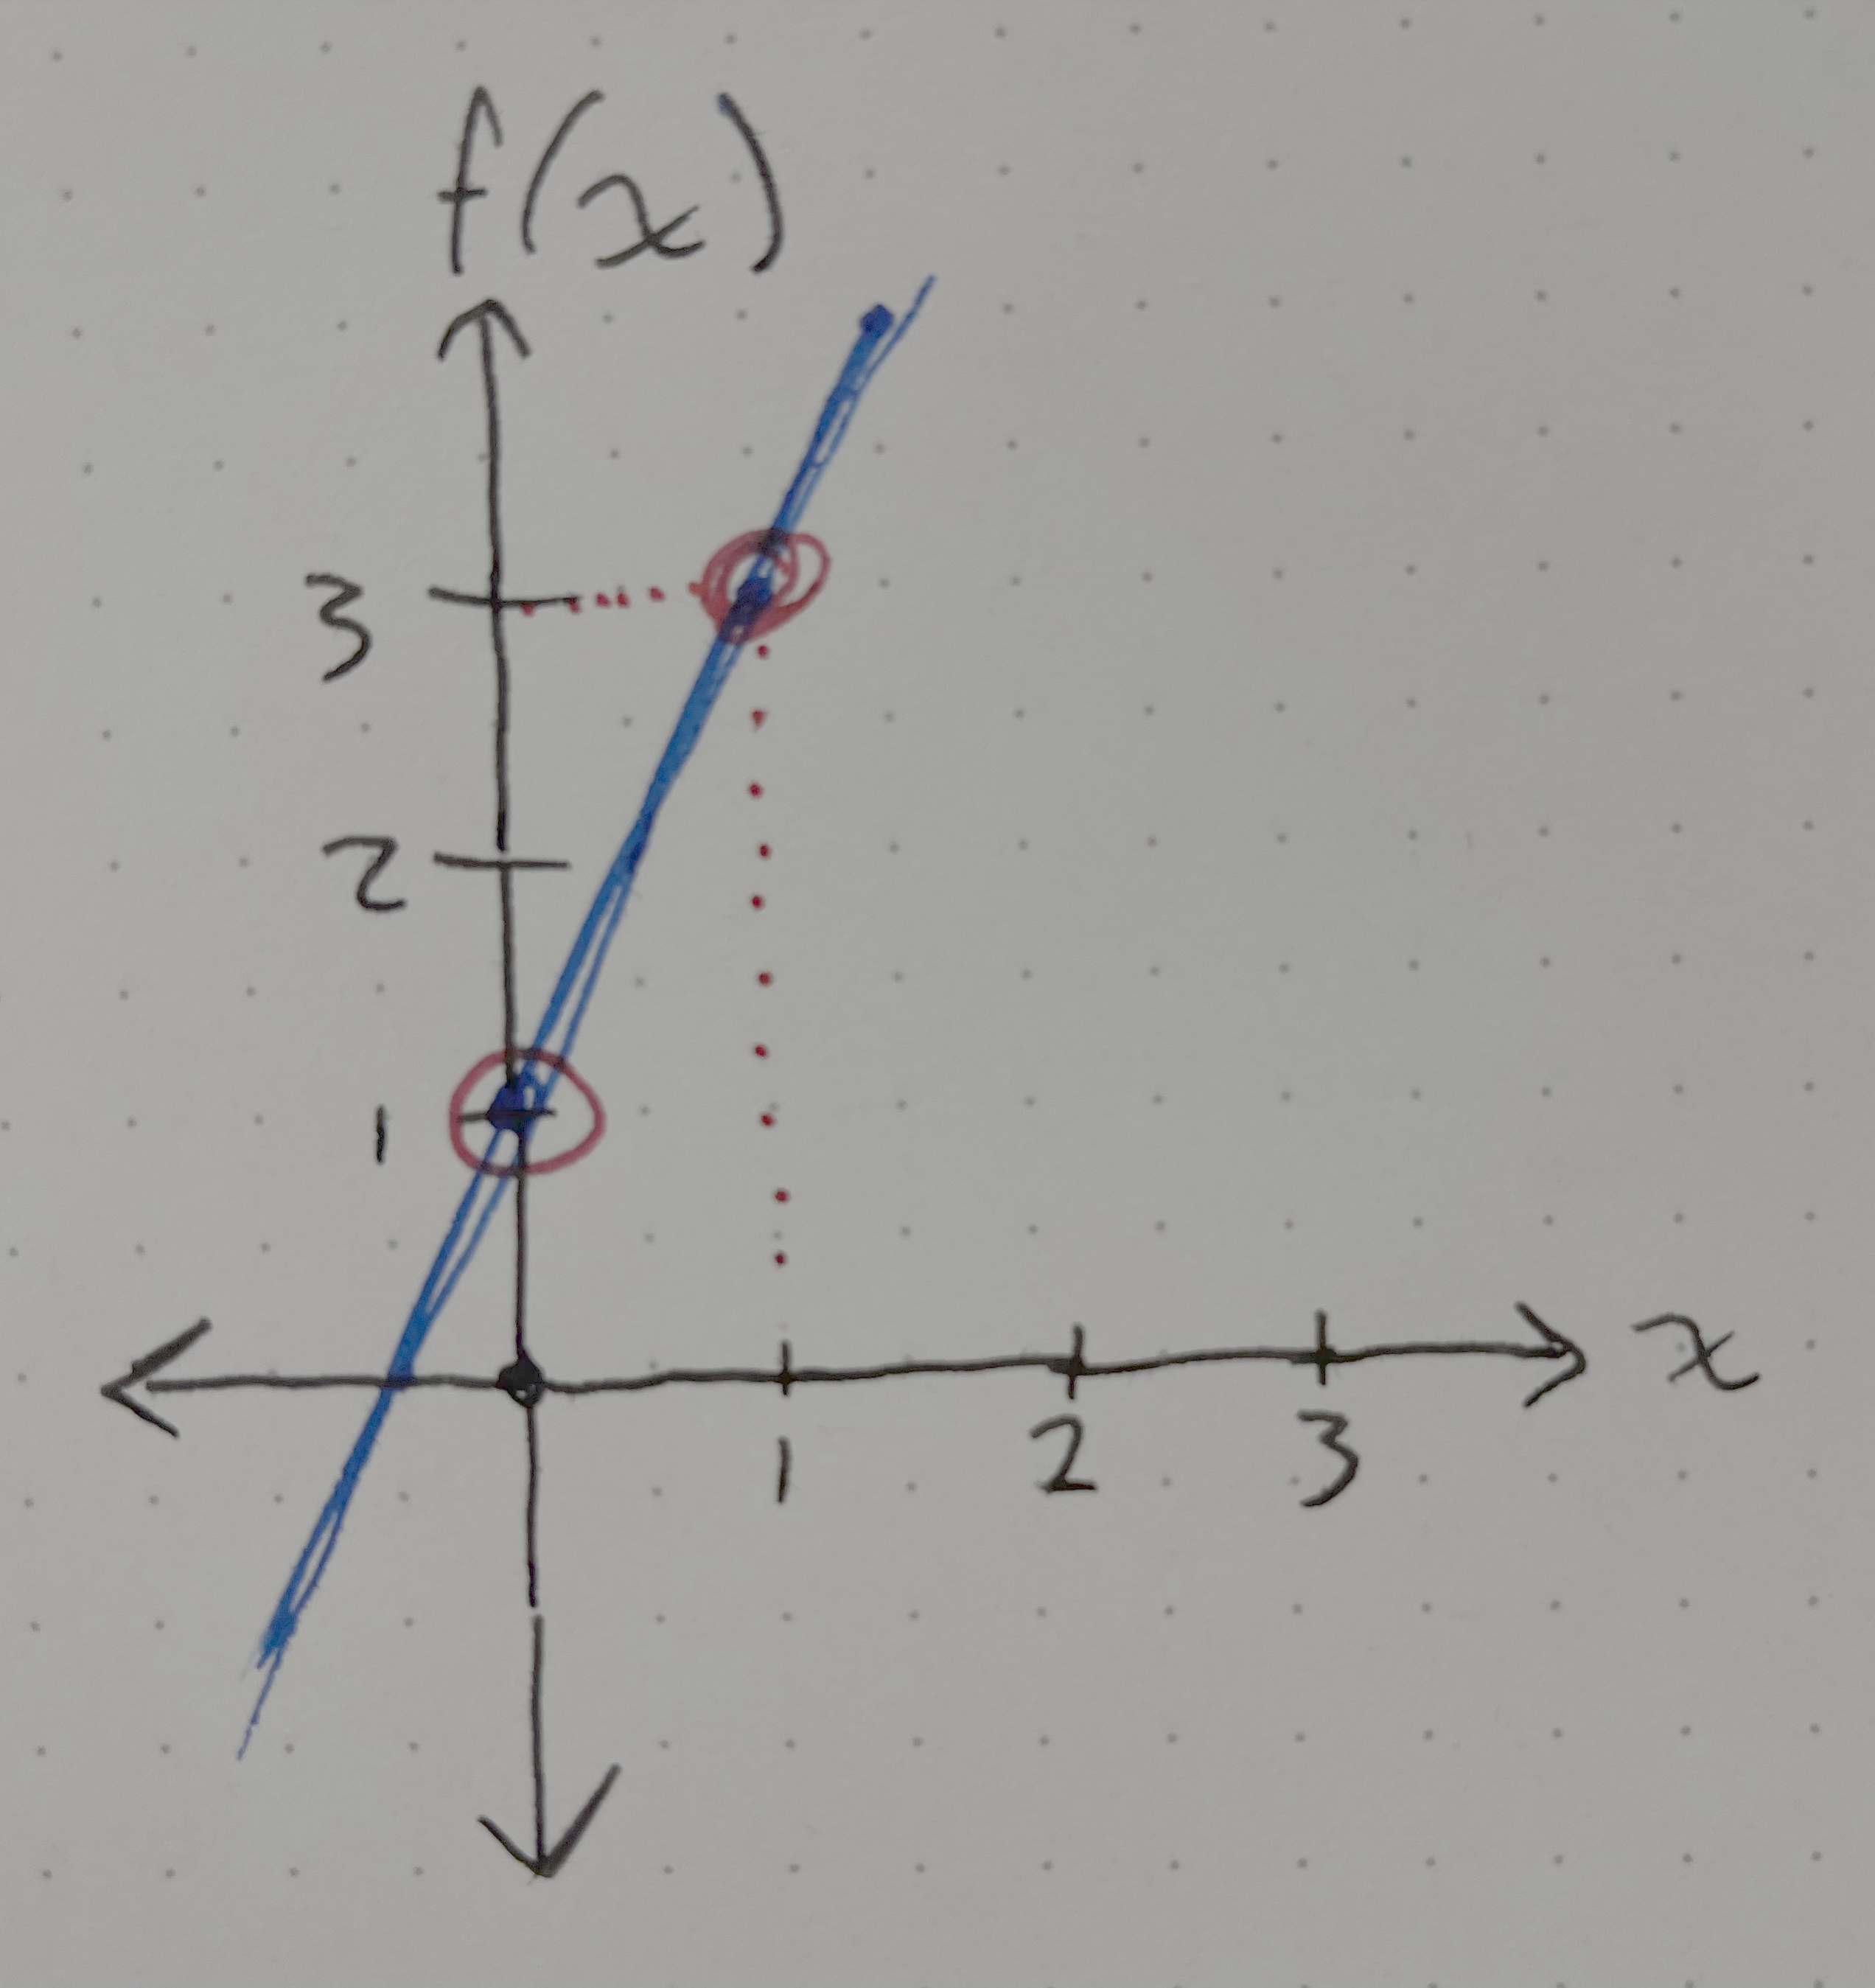
\includegraphics[scale=0.08]{fxis2xp1.png}
}{
    
    \\
        \part What is the expected value of \texttt{f( 0 )}? 
            \\
            \Soln{1, easy to see on the \texttt{f(x)} axis}
        \part What is the expected value of \texttt{f(f( 0 ))}?
            \\
            \Soln{3, \texttt{f(0)} equals \texttt{1}, so it must be the case that \texttt{f(f(0)) = f(1)}. \texttt{f(1)} is shown with dashed lines on the graph, value is \texttt{3}}
        \part Is \texttt{f(f( 0 ))} a recursive call?
            \\
            \Soln{No. This is a nested call. Those are different topics. You have had lots of experience with nested calls by this point in the semester.}
        \part What is the best representative type for \texttt{x} and \texttt{f(x)} if we wanted to write code about this?
            \\
            \Soln{\texttt{double} or \texttt{float} would be preferred. The graph is continuous and includes values like $\pi$. If we used an \texttt{int} then we wouldn't have a line, we would just have dots at each relevant whole number.}
} %end twocol
        \part Author code for the pictured function. Use a function with a reasonable name and parameters as needed. Do not use \texttt{cin}:
            \\
            \Soln{ see below in black. }
    \begin{verbatim}
    double f( double x )
    { 
        return 2 * x + 1;
    }
    \end{verbatim}

        \part What library is used for testing? How do we include it in our code?
            \\
            \Soln{\#include$\langle$cassert$\rangle$}
        \part Author assertions for \texttt{f( 0 )} and \texttt{f(f( 0 ))}
            \\
            \Soln{
            There are so many ways to do this. I'll keep the tight solutions here. \\
            assert( f(0) == 1 ); \\
            assert( f(f(0)) == 3 );
            }
        \part Now that you've done this on paper, go check your work in a coding environment of your choosing. 
            \\ \SolnNo % \Soln{this question is subjective}
    \end{parts}

    \newpage
    

\question{Reading Functions: guided:: } The questions on this page ask about the recursive \texttt{g} function defined below:
\begin{verbatim}
string g( string x )
{
    string y = "";
    switch ( x.length( ) % 3 ) {
    case 0:
        y += "Alpha";
        break;
    case 1:
        y += "Bravo";
        break;
    case 2:
        y += "Charlie";
        y = "break";
    case 3:
        y += "Delta";
    default:
        y = "Echo" + y;
    }
    return y;
}
\end{verbatim}

    \begin{parts}
        \part What is the value of \texttt{ g( "" ) }?
            \\
            \Soln{ \texttt{"Alpha" } }
        \part What is a good test for \texttt{ g( "" ) }?
            \\
            \Soln{ \texttt{assert( g( "" ) == "Alpha" );} }
        \part What is a good test for \texttt{ g( "3" ) }?
            \\
            \Soln{ \texttt{assert( g( "3" ) == "Bravo" );} }
        \part What is a good test for \texttt{ g( "ab" ) }?
            \\
            \Soln{ \texttt{assert( g( "ab" ) == "EchobreakDelta" );} }
        \part What is a good test for \texttt{ g( "san" ) }?
            \\
            \Soln{ \texttt{assert( g( "san" ) == "Alpha" );} }
        \part What are valid argument values for \texttt{x} that would get \texttt{g} to return the string \texttt{"EchoDelta"}? Describe the requirements of \texttt{x} in words.
            \\
            \Soln{This is never possible for the current defined function \texttt{g}, the switch is subject to even-divisibility of the input string \texttt{x} by value \texttt{3} it is bound on 0 to 2 inclusive.}
    \end{parts}
    \newpage


\question{Reading Functions: guided:: } The questions on this page ask about the recursive \texttt{foo} function defined below:
\begin{verbatim}
string foo( string x ) {
    string result = "";
    if ( x != "" ) {
        istringstream y( x );
        string z, remaining;
        getline( y, z, ':' );
        getline( y, remaining );
        if ( z.length() % 2 == 0 ) {
            result = z + ">" + foo( remaining );
        } else {
            result = foo( remaining );
        } 
    }
    return result;
}
\end{verbatim}

    \begin{parts}
        \part What is the base case of the \texttt{foo} function? What is a good test for this function call?
            \\
            \Soln{\texttt{assert( foo( "" ) == "" );}}
        \part What is expected result of \texttt{foo( "hi:there:sup:dude" )}?
            \\
            \Soln{ \texttt{"hi>dude>"} }
         \part What is expected result of \texttt{foo( ":1:23" )}?
            \\
            \Soln{ \texttt{">23>"} }
        \part In your own words, describe the goal of the \texttt{foo} function. This is looking for you to define your own understanding and is not looking for an exact answer.
            \\
            \Soln{Something about splitting a string by `:' delimiters, and keeping only the even length strings. Not looking for an exact answer, but making sure we have our own conceptual model of the function. \textbf{During exams, it is often a good idea to figure out what a function does at a high level before trying to work through the code by hand for a specific set of inputs.} }
        \part Write down notes about \texttt{getline} (shown above) vs \texttt{>>} (not shown).
            \\
            \SolnNo
    \end{parts}
    \newpage


    
\question{Reading helper functions and writing functions: self-study} Use the provided \texttt{isOdd} function to solve a more interesting problem of your own choosing. (hint provided at top of next page)

\begin{verbatim}
bool isOdd( int y ) {
    if ( y == 0 ) return false;
    // ask yourself if the `else` is necessary here
    else if ( y == 1 || y == -1 ) return true;
    if ( y > 0 ) return isOdd( y - 2 );
    return isOdd( y + 2 );
}
\end{verbatim}

Ideas for approach:
    \begin{parts}
        \part Describe the task that could call \texttt{isOdd}
        \part Define the task well and draw pictures of expected inputs and outputs
        \part write the a function to solve your task. Be sure to call \texttt{isOdd} in your function.
        \part now that you have completed this on paper, validate it in VSCode. Debug on paper as needed.
    \end{parts}
    \\
    \SolnNo
    \newpage
    \textbf{HINT FOR PREVIOUS PAGE: try appending a ``.'' to strings that are odd length, try counting the number of odd values in an array (available in solutions code), try removing all odd values from a vector, try it with a loop, try it with recursion, try it with a vector of structs that have ints rather than just a vector of int (available in solutions code).}


\question{writing functions: self-study} Use this page to work through a function (or collection of functions) of your own design. If you can't think of a problem worth solving with a function, ask a peer, ask a member of the course staff (in office hours or on EdStem), ask an AI that you trust. Consider the same kind of ``ideas for approach'' that are described on the previous page.
    \\
    \SolnNo
    \newpage

\question{(static) arrays[\; ]: guided::} The following questions rely on the provided code
\begin{verbatim}
void prependDont( string x[][2], unsigned int len ) {
    for ( unsigned int i = 0 ; i < len ; i++ ) {
        x[i][1] = x[i][0];
        x[i][0] = "Don't";
    }
}
void printMat( string x[][2], unsigned int len ) {
    for ( unsigned int row = 0 ; row < len ; row++ ) {
        for ( unsigned int col = 0 ; col < 2 ; col++ ) {
            if ( col != 0 ) { cout << " "; }
            cout << x[row][col];
        }
        cout << endl;
}   }
int main() {
    string mat[4][2] =  {
        { "stop", "overthinking" },
        { "think" }, { "procrastinate" }, { "give up" }
    };
    // YOUR CODE HERE
}
\end{verbatim}

\begin{parts}
    \part What is the value of \texttt{mat[0][1][2]} for the \texttt{mat} defined in \texttt{main}?
        \\
        \Soln{\texttt{'e'}}
    \part What does \texttt{prependDont} function do?
        \\
        \Soln{Prepends the word \texttt{"Don't"} to each row of the matrix, limited to the \texttt{len} provided. Uses pass-by-reference to modify the parameter \texttt{x}.}
    \part What does the \texttt{printMat} function do?
        \\
        \Soln{prints the first \texttt{len} rows of the matrix for you. It happens to use pass-by-reference, but this particular function doesn't modify the matrix.}
    \part What do you need to write in \texttt{// YOUR CODE HERE} to produce the following result using both of the functions provided? (yes, it's a silly thing to do, but it is something you have the skills for)
        \\
\begin{verbatim}
Don't stop
think
\end{verbatim}
\\
\Soln{ \\
prependDont( mat, 1 ); \\
printMat( mat, 2 ); \\
\textbf{Like we noted during the \texttt{foo} question, during exams, it is often a good idea to figure out what a function does at a high level before trying to work through the code by hand for a specific set of inputs. On an exam, you might only see this question and not parts (b) and (c).\\OBSERVE that pass by reference means prependDont will change mat for us\\OBSERVE that using numbers smaller than 4 is valid and causes specific behavior. }
}
\end{parts}
    \newpage

\question{(static) arrays[\; ]: self study::} Construct your own problem and seek resources as needed. \textbf{Try to do something where the length matters and the use of pass-by-reference matters}
    \\
    \SolnNo
    \newpage

\question{Vectors: guided::} This page explores the problem of removing every even indexed element from vector of structs through a function named \texttt{rmEvenIndices}. An example is given below.
\begin{verbatim}
struct Hand {
    int value;
    string details; 
};    
vector<Hand> table;
table.push_back( { 11, "double down" } );
table.push_back( { 17, "troublesome hand" } );
table.push_back( { 21, "blackjack" } );
table = rmEvenIndices( table ); // index 0 and index 2 removed
// remaining: { 17, "troublesome hand" }
\end{verbatim}

    \begin{parts}
        \part What are three good tests that you can write for the final \texttt{table} after \texttt{rmEvenIndices} is called shown above in a comment? 
            \\
            \Soln{ \\
            \texttt{assert( table.size() == 1 );} \\
            \texttt{assert( table.at( 0 ).details == "troublesome hand" );} \\
            \texttt{assert( table.at( 0 ).value == 17 );} \\
            there are other options, but they are less obvious
            }
        \part Which of the following vector methods are likely helpful in solving \texttt{rmEvenIndices}: \textttt{at}, \texttt{begin}, \texttt{back}, \texttt{pop\_back}, \texttt{push\_back}, \texttt{insert}, and \texttt{erase}? Why? (not looking for exact answer, just getting out ideas.)
            \\
            \Soln{``\texttt{pop\_back}'' and ``\texttt{erase}'' feel like good candidates. It might be possible with just ``\texttt{at}''.}
        \part Implement \texttt{rmEvenIndices}. Start with the function singature, move to psuedo-code and finally write a working function. It can be recursive, it can use as many or as few of the methods described. Aim for something that is easy to read.
            \\
            \Soln{ there are MANY valid answers, below is just one of them. I write a few others in the published solution code}
            \begin{verbatim}
vector<Hand> rmEvenIndices1( vector<Hand> table ) {
    // using .at and .push_back
    vector<Hand> result;
    // note how this skips over the odds
    for ( unsigned int i = 1 ; i < table.size( ) ; i += 2 ) {
        result.push_back( table.at( i ) );
    }
    return result;
}
            \end{verbatim}
        
    \end{parts}
    \newpage

\question{Vectors: self study::} Construct your own problem and seek resources as needed. \textbf{to optimize study, find a problem that uses the methods not used in the previous problem.}
    \\
    \SolnNo
    \newpage

\question{Streams: warm up} 
    \begin{parts}
        \part Describe the difference between and input stream and output stream.
            \\
            \Soln{Input streams like \texttt{cin} are used to read data from the stream into the code. Output streams like \texttt{cout} are used to write data from the code to the stream.}
        \part Describe the difference between the following:
            \begin{itemize}
                \item \texttt{x >> y}
                \item \texttt{getline( x, y )}
                \item \texttt{getline( x, y, z )}
            \end{itemize}
            \\
            \Soln{
            \begin{itemize}
                \item In all of these cases \texttt{x} is an input stream that we are reading from. they all work on \texttt{cin}, \texttt{istringstream}, and \texttt{ifstream}. 
                \item  \texttt{getline} requires that \texttt{y} is a string, while \texttt{>>} allows \texttt{y} to be another type and will do type conversions of the string data for us if it can.
                \item  \texttt{x >> y} reads until the first whitespace (space, tab, NEW\_LINE), shoves that data into \texttt{y} without the whitespace attempting type conversions as needed. \textbf{It STOPS the read head BEFORE the white space (often want to pair with \texttt{ingore})}
                \item  \texttt{getline( x, y )} reads until the first NEW\_LINE, shoves that data into \texttt{y} without the new-line as a string. \textbf{It STOPS the read head AFTER the new-line}
                \item  \texttt{getline( x, y, z )} reads until the first \texttt{char z}, shoves that data into \texttt{y} without the \texttt{char z} as a string. \textbf{It STOPS the read head AFTER the \texttt{char z}}
            \end{itemize}}
        \part Let there be an input stream named \texttt{x} with the following data:
        \begin{verbatim}
            hello   my name is
            Gregor
            and more stuff is here
        \end{verbatim}

        We run the following code:
        \begin{verbatim}
            string y0, y1, y2;
            x >> y0; // y0 is "hello"
            // CHANGE CODE
            getline( x, y1, 'g' );  // y1 is "   my name is<NEW_LINE>Gre
            getline( x, y2 );  // y2 is "or"
        \end{verbatim}
            State in your own words why each of the following are true
            \begin{itemize}
                \item \texttt{y0} does not have a space at the end.
                \item \texttt{y1} has a three spaces at the beginning. (followup: what could you write in ``CHANGE CODE'' to remove that whitespace?)
                \item \texttt{y1} includes a newline in the middle of it
                \item \texttt{y1} doesn't end with the letter `g'.
                \item \texttt{y2} doesn't begin with the letter `g'.
                \item \texttt{y2} doesn't end with a newline.
            \end{itemize}
            \Soln{See explanations in previous question to answer these questions. Explore it in your prefered coding environment to better understand this topic.}
        \part What is different about opening an \texttt{ifstream} vs an \texttt{ofstream}?
            \\
            \Soln{If you open an \texttt{ofstream} and the file does not already exist, the library will make the file for you as long as it has permission to do so in that location on your computer. This is not true for \texttt{ifstream}. Note, you still need to do a check that the file is open due to system permissions and other uncommon issues.}
        \part Why is it important to close a file stream?
            \\
            \Soln{Failure to close any file stream, can result in a security vulnerability that allows bad actors to mess with your data. Specific to output, failure to close \texttt{ofstream} my lead to the data you wrote not actually being saved to the file, so your code took time to run, but didn't really get the job done.}
    \end{parts}
    \newpage

\question{Streams: self study::} Construct your own problem and seek resources as needed.\textbf{NOTE: streams covered this semester include \texttt{iostream}, \texttt{fstream}, and \texttt{sstream}. Note the provided array problem tests \texttt{getline}, consider writing a problem that works with input and output streams and uses \texttt{>>} instead of \texttt{getline}.  (hint provided at top of
next page)}
    \SolnNo
    \newpage

\textbf{HINT FOR PREVIOUS PAGE} Write a function, given two file names as strings, read data from the first file, write the data to the second file, but remove all lines which begin with the phrase ``\texttt{COMMENT :}''. Do not change the first file. Use best practices to open and close files.
\\
\Soln{code available in solution code document... be sure to write a valid in.txt file and open the out.txt file to validate if the code actually works.}
\question{Structs/Instances: warm up} 
    \begin{parts}
        \part Following best-practice in C++, should a \texttt{struct} contain member functions? 
            \\
            \Soln{No. Sure, you can technically do it, but it's strongly NOT recommended, use a \texttt{class}  instead.}
        \part Following best-practice in C++, should a \texttt{struct} contain ``private'' data? 
            \\
            \Soln{No. Sure, you can technically do it, but structs have default access modifier ``public'' and should really only have public non-function data. If you want private data, use a \texttt{class} instead.}
        \part When passing a struct to a function, does it default to pass-by-value or pass-by-reference?
            \\
            \Soln{pass-by-value. Only arrays are pass-by-reference.}
        \part When passing an array of structs to a function, does it default to pass-by-value or pass-by-reference? Why?
            \\
            \Soln{pass-by-reference. arrays are pass-by-reference. It doesn't matter what the type of the elements of the array are, it's still an array.}
        \part When passing a struct to a function that contains an array as a data member, does it default to pass-by-value or pass-by-reference? Why?
            \\
            \Soln{pass-by-value. The full struct is passed, a struct is not an array even if it holds an array inside it.}
         \part Consider a struct that has an array as a data member accessed \texttt{instance.array}, when calling a function with argument \texttt{instance.array}, does it default to pass-by-value or pass-by-reference? Why?
            \\
            \Soln{pass-by-reference. We are no longer passing the struct to the function, we are passing the internal array to the function.}
        \part When passing an array of structs to a function that contains an array as a data member, does it default to pass-by-value or pass-by-reference? Why?
            \\
            \Soln{pass-by-reference. Note a few important points here:
            \begin{enumerate}
                \item The internals of the struct having their own arrays does not matter. That is a mislead in the question. \textbf{Learning what is and is not important when reading a question can save you a lot of time during an exam. Ask on \hyperlink{https://edstem.org/us/courses/72170/discussion}{EdStem} for more examples from your past exams.}
                \item The type of each element of the outer array does not matter.
                \item We are passing an array to a function. Arrays are pass-by-reference.
            \end{enumerate}}
        
    \end{parts}
    \newpage

\question{Structs/Instances: self study::} Construct your own problem and seek resources as needed.
    \\
    \SolnNo
    \newpage

\question{Classes/Objects: guided::} let us play a game with friends. Before reading further decide on who will be the ``game lead(s)'' and ``adventurer(s)'' (need at least one of each). Now, only the game lead(s) should read further....
\begin{enumerate}
    \item Opening dialog read by the game lead(s): ``In the heart of the arcane sanctum, a series of ancient number glyphs lie etched into stone boxes, each pulsing faintly with enchanted light. A mysterious spell binds them—an enchantment I know well, yet am bound by oath and magic to speak nothing of its nature. \\
Your quest is thus: brave the puzzle, unravel the pattern, and uncover the hidden magic woven within. Only through trial and cunning can you pierce the veil and reveal the secret of the spell. Will you accept this challenge, adventurer?'' (credit ChatGPT)
    \item Explain to the adventurer(s) their available moves: 
    \begin{enumerate}
        \item ``explore a new glyph''
        \item ``view the glyph''
        \item ``apply pressure to the the glyph \texttt{<quantify with a number>}''
        \item ``reduce pressure to the the glyph \texttt{<quantify with a number>}''
        \item attempt to describe the magic spell
    \end{enumerate}
    \item Don't share the following information with the adventurer(s). The game lead(s) available moves are as follows:
    \begin{enumerate}
        \item if the adventurer wishes to explore a new glyph, ignore all known number boxes, call the default constructor to make a new object to observe.
        \item if the adventurer wishes to view the glyph, you must tell them the current number.
        \item if the adventurer applies pressure to the glyph, you must call the setter with a positive number and apply the rules of the \texttt{\_magic} function. Tell the player when you are ready to continue, but do not tell them the value of the glyph or show them any of your math.
        \item if the adventurer reduces pressure to the glyph, you must call the setter with a negative number...
        \item if the adventurer describes the magic spell incorrectly, you must tell them to keep playing the game. \textbf{Add any lore you wish.}
        \item if the adventurer describes the magic spell correctly, make up your own ending for the game.
    \end{enumerate}
    \item all code is on the next page for the game lead(s) to use to facilitate the game.
    \item after the game ends, review the code together. Review topics like \textbf{default vs parameterized constructors}, \textbf{data members (attributes) vs member functions (methods)}, \textbf{public vs private (access modifiers)}, \textbf{getters vs setters}, \textbf{class vs object}, the differences in application and best practices between \textbf{struct vs class}. Write a \textbf{parameterized constructor} for the \texttt{NumBox} class that sets the value and calls the private \texttt{\_magic} function.
\end{enumerate}
\newpage
\begin{verbatim}
class NumBox {
public: 
    NumBox();
    float getValue( );
    void setValue( float value );
private:
    float _value;
    unsigned short _accessCount;
    void _magic( );
};
NumBox::NumBox() {
    _accessCount = 0;
    _value = 0;
}
float NumBox::getValue( ) {
    _accessCount++;
    return _value;
}
void NumBox::setValue( float value ) {
    _accessCount++;
    _value = value;
    _magic();
    return;
}
void NumBox::_magic( ) {
    int i = _value; 
    if ( i % 2 == 1 ) _value = i - 1;  
    // ADVANCED PLAY ONLY:
    // if ( i % 2 == 1 ) _value = _accessCount - 1;
    else _value = i;
    _value += 0.5;
}
// // >>>>>>>>>>>>>>>>>>>>>>>>>>>>>>>>>>>>>>>>>>>>>>>>>>>>>>>>>>>>>>>>>
// ADVANCED PLAY ONLY: add this public member function.
// unsigned short NumBox::getAccessCount( ) {
//     // return _accessCount++;  // kind of advance post-increment... 
//     unsigned short res = _accessCount;
//     _accessCount++;
//     return res;
// }  // <<<<<<<<<<<<<<<<<<<<<<<<<<<<<<<<<<<<<<<<<<<<<<<<<<<<<<<<<<<<<<
\end{verbatim}
    \Soln{the code is available for download. You can write a small driver to play against the computer. You can take turns writing new \texttt{\_magic} functions to see if the other player can guess your magic spell(s).}
    \newpage
    
\question{Classes/Objects: self study::} Construct your own problem and seek resources as needed. \textbf{NOTE: vectors and their member functions are great example of a well defined class. The \texttt{vector} class defines a series of member functions for you to use to access complex memory without having to worry about how the memory is handled}
    \\
    \SolnNo
    \newpage

\question{nesting concepts: warmup}
    \begin{parts}
        \part What data types default pass-by-reference?
            \\
            \Soln{arrays}
        \part What data types default pass-by-value?
            \\
            \Soln{all other data types}
        \part What data types use dot-notation? Give an example.
            \\
            \Soln{struct instances derived from structs (sometimes called objects) and objects derived from classes. RECALL best-practice is that all struct members are public while classes make encapsulate data members (attributes) as private and instead access and manipulate the data through public member functions (methods) called getters or setters. This includes imported classes like ``vector'', ``string stream'', and ``file stream''. \\
            e.g\\ 
            \texttt{ vector<int> v ; v.push\_back( 5 ); }}
        \part What data types use bracket-notation? Give an example.
            \\
            \Soln{arrays and strings \\ e.g.\\ \texttt{ string arr[5] = { "hello", "there" } ; arr[0][4]; }}
        \part Following C++ best practice, how do you access data from a struct instance? Give an example.
            \\
            \Soln{Use dot notation. Access the data directly.\\  e.g. let MyStruct be a defined struct with int member ``x''\\ \texttt{ MyStruct instance = { 4 }; cout << instance.x << endl; }}
        \part Following C++ best practice, how do you access data from a object? Give an example.
            \\
            \Soln{Use dot notation. Access the encapsulated private data member (attribute) through a public member function (attribute)[getter]. \\ e.g. let MyClass be a defined class with private int data member ``\_y'' and public member function ``getY'' and a paramterized constructor \\ \texttt{ MyClass object(4); cout << object.getY( ) << endl; }}
    \end{parts}
    \newpage
    
\question{Nesting concepts: self study::} Construct your own problem and seek resources as needed. \textbf{NOTE: any of the self-studies earlier in this packet are great candidates to practice nesting. A pinnacle problem to solve may involved a class that encapsulates a vector of 2-D arrays of structs that include strings resulting in accesses requirements like:\\ \\ \texttt{o.getVector().at( 0 )[ 1 ][ 2 ].stringMember[ 3 ];}\\ \\ You could also consider having streams instead of strings at the final layer like:\\ \\ \texttt{getline( o.getVector().at( 0 )[ 1 ][ 2 ].streamMember, someString, ':' );}}\\ \\Then consider different orderings of this nesting and various functions to deal with pass-by-reference vs pass-by-value behavior. Throw in a class for good measure. 
\\
\\
\textbf{RECALL: The questions in this study guide are designed to be difficult and help you identify knowledge gaps that warrant further study.} 
    \\
    \SolnNo
    \newpage

\end{questions}
\end{document}
